\documentclass{beamer}

\usetheme{Warsaw}
\usecolortheme{crane}

\usepackage[utf8]{inputenc}
\usepackage[english]{babel}

\usepackage{listings}
\lstset{%
  basicstyle=\ttfamily\footnotesize,
  showstringspaces=false,
}

\graphicspath{{images/}}

\title[Intro to Git]{Introduction to Git}
\author{Armin Leuprecht}
\institute
{
  Wegener Center for Climate and Global Change\\
  University of Graz
}
\date[2016-07-28]{T4S, 28$^{th}$ July 2016}

% \AtBeginSection[]
% {
%   \begin{frame}
%     \frametitle{Table of Contents}
%     \tableofcontents[currentsection]
%   \end{frame}
% }


\begin{document}
\beamertemplatenavigationsymbolsempty

\begin{frame}
  \titlepage
\end{frame}

\section[VCSs]{Version control systems}
\begin{frame}
  \frametitle{Version control}
  \framesubtitle{Record the history of files}

  Why do you want to use a VCS?
  \begin{itemize}
  \item revert to previous file versions
  \item compare changes over time
  \item find out who modified something
  \item easy recovery when things screw up
  \end{itemize}

  Why do you have to use a VCS?
  \begin{itemize}
    \item reproducibility
    \item transparency
    \item confirmability
  \end{itemize}
\end{frame}

\begin{frame}[fragile]
  \frametitle{Types of VCSs}
  \begin{itemize}
  \item<1-> Manual version control
  \item<2-> Local VCS
  \item<3-> Centralized VCS
  \item<4-> Distributed VCS
  \end{itemize}

  \begin{overprint}
    \onslide<1>
    \begin{alertblock}{Manual VC}
      \emph{No good idea -- very error prone}
      \begin{lstlisting}[language=bash]
        ...
        v179_20150115_ReLoClimWrittenPublications.docx
        v180_20150115_ReLoClimWrittenPublications.docx
        v180b_20150115_ReLoClimWrittenPublications.docx
        v181_20150205_ReLoClimWrittenPublications.docx
        v182_20150205_ReLoClimWrittenPublications.docx
        v183_20150206_ReLoClimWrittenPublications.docx
      \end{lstlisting}
    \end{alertblock}

    \onslide<2>
    \begin{block}{Local CSV}
      \begin{minipage}{.5\linewidth}
        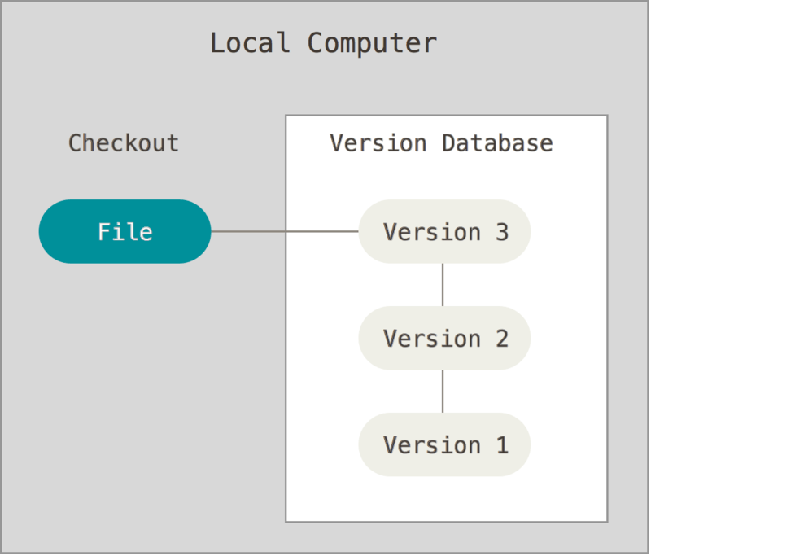
\includegraphics[width=\textwidth]{local}        
      \end{minipage}\hfill
      \begin{minipage}{.5\linewidth}\small
        Pros:
        \begin{itemize}
          \item fast and easy for single user/machine
        \end{itemize}
        Cons:
        \begin{itemize}
          \item difficult administration over systems
        \end{itemize}
        Examples: rcs
      \end{minipage}

    \end{block}

    \onslide<3>
    \begin{block}{Centralized VCS}
      \begin{minipage}{.5\linewidth}
        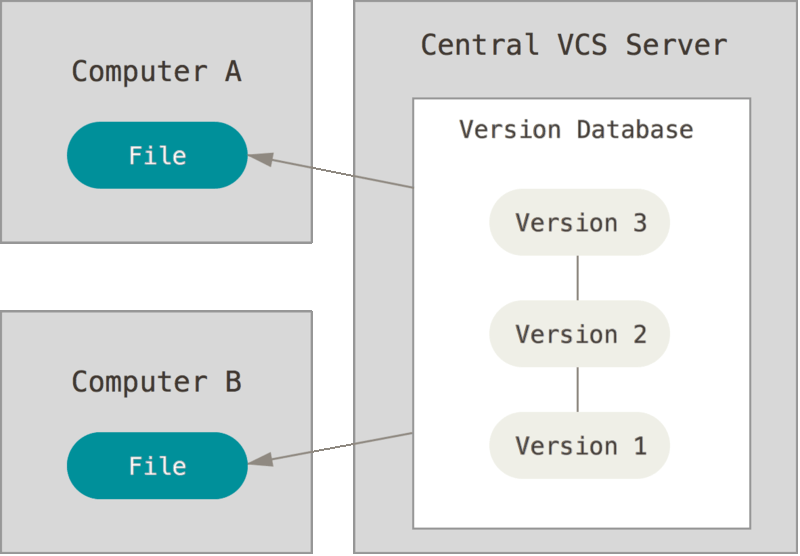
\includegraphics[width=\textwidth]{centralized}
      \end{minipage}
      \begin{minipage}{.45\linewidth}\small
        Pros:
        \begin{itemize}
          \item easy administration
          \item fine-grained control
        \end{itemize}
        Cons:
        \begin{itemize}
          \item single point of failure
        \end{itemize}
        Examples: cvs, subversion
      \end{minipage}
    \end{block}

    \onslide<4>
    \begin{exampleblock}{Distributed VCS}
      \begin{minipage}{.5\linewidth}
        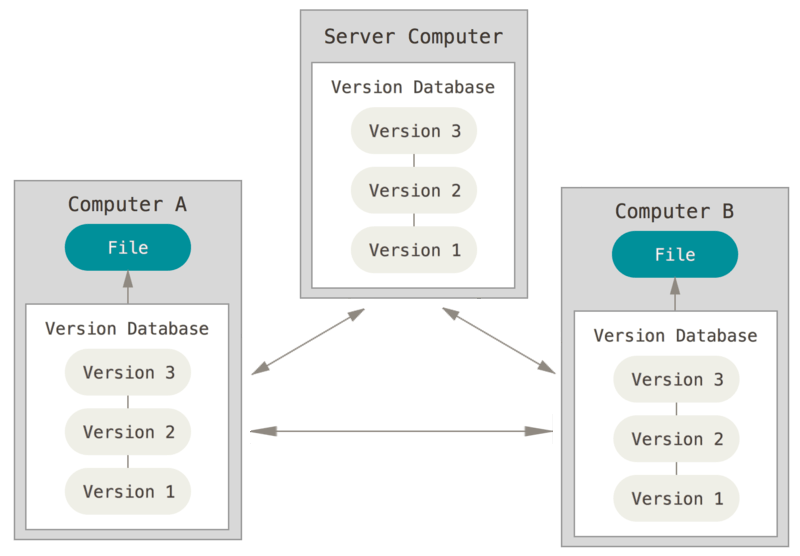
\includegraphics[width=\textwidth]{distributed}
      \end{minipage}
      \begin{minipage}{.45\linewidth}\small
        Pros:
        \begin{itemize}
          \item extremely fast
          \item full mirror of the repository
          \item several workflows
        \end{itemize}
        Cons:
        \begin{itemize}
        \item large binary files/history
        \end{itemize}
        Examples: Git, Mercurial, Bazaar
      \end{minipage}
    \end{exampleblock}

  \end{overprint}
    
\end{frame}

\section[Git Basics]{Git Basics}
\begin{frame}
  \frametitle{History}
  Created in 2005 for the development of the Linux kernel

  Naming (by Linux Torvalds) -- depending on your mood
  \begin{itemize}
    \item random three-letter combination that is pronounceable, and not
      actually used by any common UNIX command.  The fact that it is a
      mispronunciation of "get" may or may not be relevant.
    \item stupid. contemptible and despicable. simple. Take your pick from the
      dictionary of slang.
    \item "global information tracker": you're in a good mood, and it actually
      works for you. Angels sing, and a light suddenly fills the room.
    \item "goddamn idiotic truckload of sh*t": when it breaks
  \end{itemize}
\end{frame}

\begin{frame}
  \frametitle{Goals}
  \begin{itemize}
    \item Speed
    \item Simple design
    \item Fully distributed
    \item Emphasis on non-linear development
  \end{itemize}
\end{frame}

\begin{frame}[fragile]
  \frametitle{Storage: Snapshots -- no diffs}
  \begin{itemize}
    \item<1-> Traditional view: list of file-based deltas
    \item<2->   Git: stream of snapshots
      \begin{itemize}
        \item more like a mini file-system
        \item very efficient when it comes to branching
      \end{itemize}
  \end{itemize}

  \centering
  \begin{overprint}
    \onslide<1>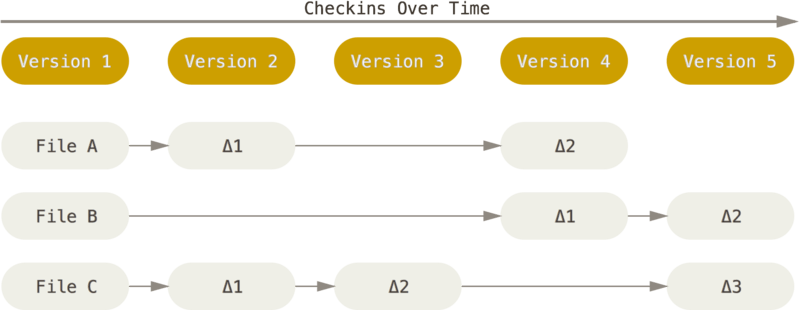
\includegraphics[width=.9\textwidth]{deltas}
    \onslide<2>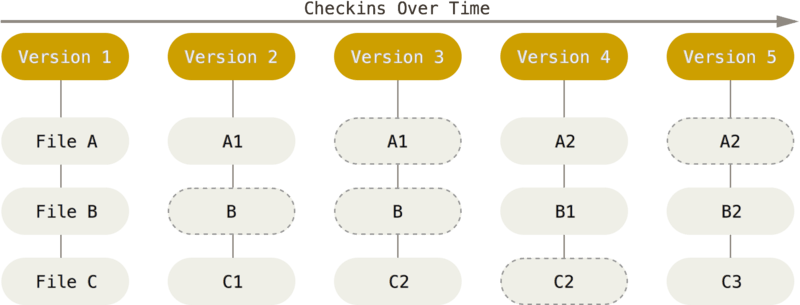
\includegraphics[width=.9\textwidth]{snapshots}
  \end{overprint}
\end{frame}

\begin{frame}
  \frametitle{Further advantages}
  \begin{itemize}
    \item Speed: nearly every operation is local
    \item Integrity: everything is checksummed
    \item Data loss: after commit and push nearly impossible
  \end{itemize}
\end{frame}

\begin{frame}
  \frametitle{The three stages}
  Every controlled file resides in one of three main states:
  \begin{itemize}
    \item modified: you have changed the file and not committed yet
    \item staged: you have marked the file to go into your next commit snapshot
    \item committed: data is safely stored in your local database
  \end{itemize}
\end{frame}

\begin{frame}
  \frametitle{Git workflow}
  \centering
  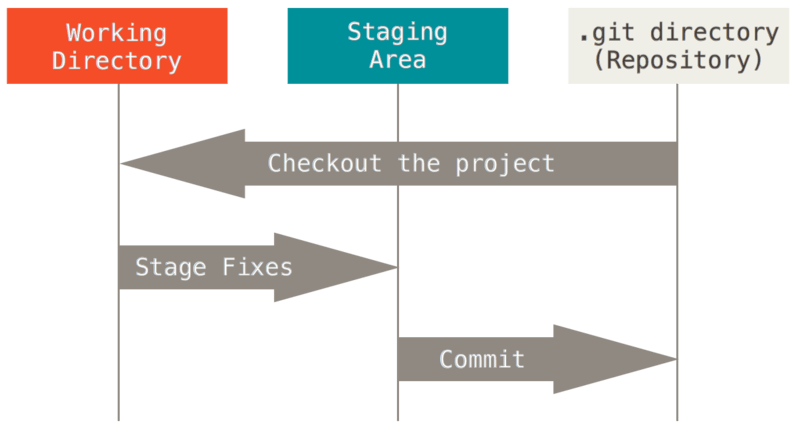
\includegraphics[width=.9\textwidth]{areas}
  \begin{itemize}
    \item modify files in working directory
    \item stage files (adding snapshots to the staging area)
    \item commit files (storing snapshots permanently in the Git directory)
  \end{itemize}
\end{frame}

\begin{frame}[fragile]
  \frametitle{Installation}
  \begin{itemize}
    \item your OS package manager (apt, yum)
    \item binary packages from Git homepage download section: \url{https://git-scm.com/downloads}
    \item get it via Git and compile it on your own (if you already have a running version):\\ 
      \verb+git clone+ \url{https://github.com/git/git}
  \end{itemize}
\end{frame}

\begin{frame}[fragile]
  \frametitle{First-time setup}
  There are three configuration places
  \begin{itemize}
    \item \verb+/etc/gitconfig+ file: system-wide for any user (written by superuser only)
    \item \verb+~/.gitconfig+ or \verb+~/.config/git/config+ file: specific to the user, can be accessed by passing the \verb+--global+ option to \verb+git config+
    \item \verb+config+ file in the Git directory (\verb+.git/config+): specific to that repository
  \end{itemize}

  Setup your identity (and your prefered editor)
  \begin{lstlisting}[language=bash]
    $ git config --global user.name "Jane Doe"
    $ git config --global user.email jane.doe@example.com

    $ git config --global core.editor emacs
  \end{lstlisting}
\end{frame}

\begin{frame}[fragile]
  \frametitle{Getting help}
  Besides many resources on the web you will get (offline) help by calling the manual pages:

  \begin{lstlisting}[language=bash]
    $ git help <verb>
    $ git <verb> --help
    $ man git-<verb>
  \end{lstlisting}
\end{frame}

\end{document}
